\documentclass[notes=show, 10pt]{beamer}
\usepackage[utf8]{inputenc}
\usepackage{xeCJK}
\usepackage{graphicx}
\usepackage {mathtools}
\usepackage{multicol}
\usepackage{utopia} %font utopia imported
\usetheme{CambridgeUS}
\usecolortheme{dolphin}

% set colors
\definecolor{myNewColorA}{RGB}{126,12,110}
\definecolor{myNewColorB}{RGB}{165,85,154}
\definecolor{myNewColorC}{RGB}{203,158,197}
\setbeamercolor*{palette primary}{bg=myNewColorC}
\setbeamercolor*{palette secondary}{bg=myNewColorB, fg = white}
\setbeamercolor*{palette tertiary}{bg=myNewColorA, fg = white}
\setbeamercolor*{titlelike}{fg=myNewColorA}
\setbeamercolor*{title}{bg=myNewColorA, fg = white}
\setbeamercolor*{item}{fg=myNewColorA}
\setbeamercolor*{caption name}{fg=myNewColorA}
\usefonttheme{professionalfonts}
\usepackage{natbib}
\usepackage{hyperref}
%------------------------------------------------------------
\titlegraphic{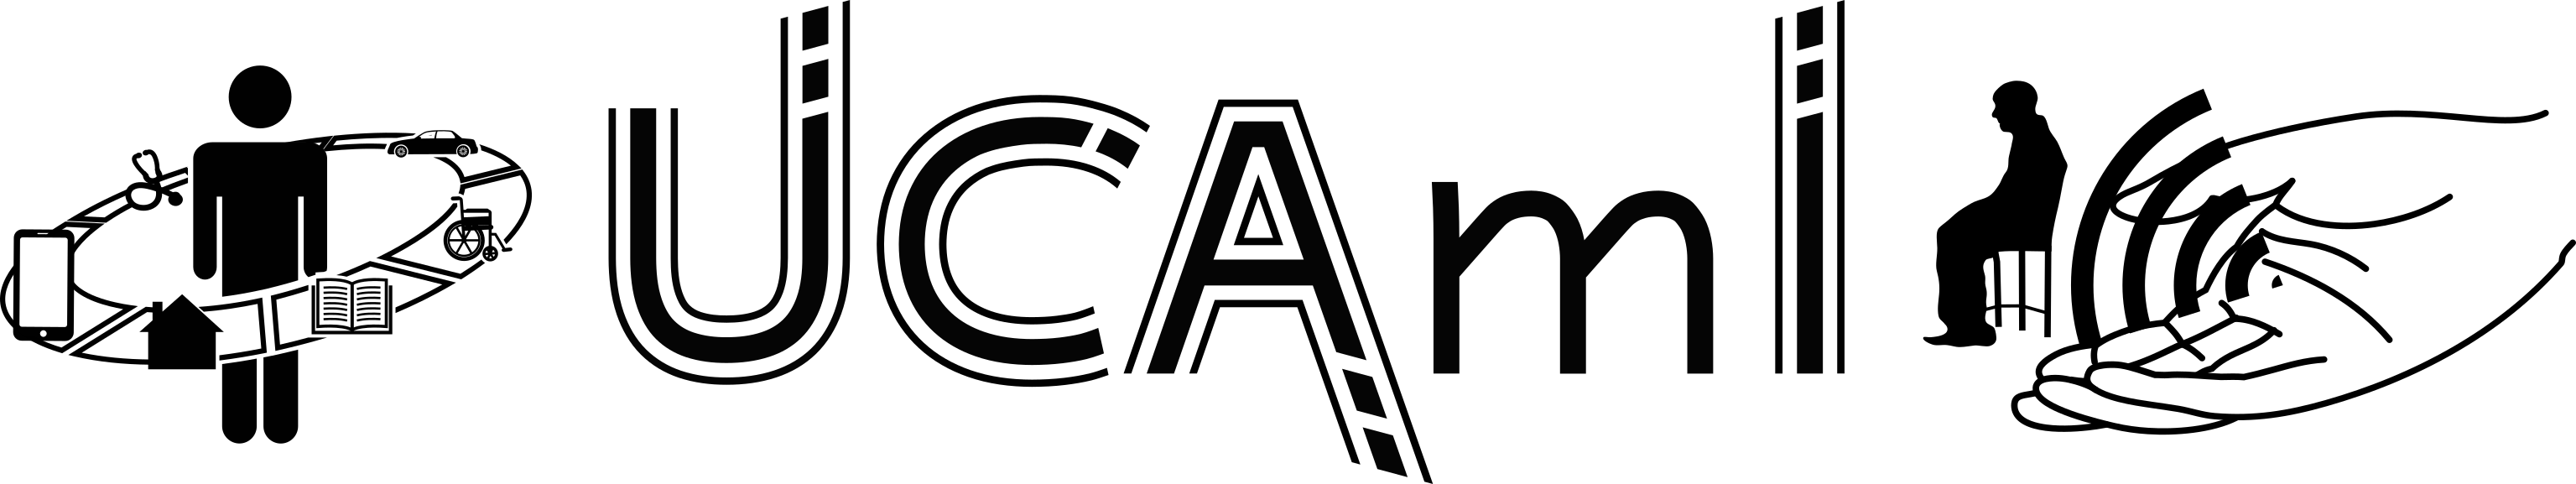
\includegraphics[height=1.5cm]{ucami2022.png}}

\setbeamerfont{title}{size=\large}
\setbeamerfont{subtitle}{size=\small}
\setbeamerfont{author}{size=\small}
\setbeamerfont{date}{size=\small}
\setbeamerfont{institute}{size=\small}
\title[UCAmI 2022]{Internet of Things (IoT)-Based System for Classroom Access Control and Resource Management}
\subtitle{(SISGERA)}
\author[Gleiston Guerrero-Ulloa]{Gleiston Guerrero-Ulloa \and Jonathan Villafuerte-Solorzano \and Michael Yánez  \and \\ Miguel J. Hornos \and Carlos Rodriguez-Domínguez}

\institute[gguerrero@uteq.edu.ec]{Technical State University of Quevedo, and University of Granada}
\date[Córdoba, November 2022]{Córdoba, November 2022}

%------------------------------------------------------------
%This block of commands puts the table of contents at the 
%beginning of each section and highlights the current section:
%\AtBeginSection[]
%{
%  \begin{frame}
%    \frametitle{Contents}
%    \tableofcontents[currentsection]
%  \end{frame}
%}
\AtBeginSection[]{
  \begin{frame}
  \vfill
  \centering
  \begin{beamercolorbox}[sep=8pt,center,shadow=true,rounded=true]{title}
    \usebeamerfont{title}\insertsectionhead\par%
  \end{beamercolorbox}
  \vfill
  \end{frame}
}
%------------------------------------------------------------

\begin{document}

%The next statement creates the title page.
\frame{\titlepage}
\begin{frame}
\frametitle{Contents}
\tableofcontents
\end{frame}
%------------------------------------------------------------

    \begin{frame}{Introduction}
        \begin{block}{What is SISGERA}
            In this work we pro-pose to SISGERA (from Spanish: SIStema de GEstión de Recursos de Aula) is a prototype of an IoT-based system that was developed as a possible and feasible solution not only to manage classroom resources but also to control access to classrooms, deploying the necessary devices in the environment. For this last purpose, and more specifically, to open the classroom door, facial recognition has been used implemented to identify the authorized person in this case a professor, who can open the classroom at a given time, according to the established class schedule. In addition, students are registered by RFID and confirmed fingerprint.\\
            Then, the \textbf{first goal} Classroom resource management aims to ensure that classroom resources are switched on for the required time.\\
            And As a consecuence, \textbf{the second goal} reduce energy consumption.\\
            And \textbf{last goal} evaluate the Test-Driven Development Methodology for IoT-Based Systems (TDDM4IoTS).\\
            SISGERA consists of a set of components that form the IoT device and a mobile application with which the user additionally controls the artefacts in the environment.
        \end{block}
    \end{frame}

    \begin{frame}{Classroom resources}
        \begin{block}{}
            The janitorial staff is in charge of opening the doors of each classroom at the beginning of the school day in the morning and closing them at the end of the school day in the afternoon.\\
            Each janitorial staff member is responsible for around 16 classrooms. In addition to managing the door locks, they are in charge of the remote controls to manage classroom equipment such as projectors and air conditioners, so they turn these on at the beginning of the day and expect to turn them off at the end of the day. However, some teachers turn them off at the end of their class session, leaving the next teacher to contact staff to turn on or turn off the equipment(s) they do not require.\\
            It is a rule that the classroom must be opened when the teacher is ready to enter, which can be a delay or rush for the janitorial staff, as one day all classrooms will be required at the same time by the respective teachers to start classes.\\
            When classes start, the teacher must register the student's attendance, and from the very first classes, students may be evaluated on their performance, and the teacher does not always identify each student, which may lead to some impersonation.
        \end{block}
    \end{frame}

    \begin{frame}{Reducing electrical energy consumption}
        \begin{block}{}
            The SISGERA prototype is implemented in a classroom at the Faculty of Engineering Sciences (FCI). The FCI offers technical courses such as Electrical Engineering, Software Engineering, Mechanical Engineering and Environmental Engineering. Each subject has only one professor in charge. Some subjects of these programs have practical hours (laboratory or field) and theoretical hours, and the professor is in charge of planning when he/she will teach the theoretical classes and when the practical classes will take place.\\
            Every day there are two shifts of classes:
            \begin{itemize}
                \item in the morning from 07h30 to 12h30 and 
                \item from 12h30 to 17h30
            \end{itemize}
            In addition, some virtual hours at the extremes of each periods.
        \end{block}
    \end{frame}
    
    \begin{frame}{Reducing electrical energy consumption...}
        \begin{block}{Academic planning...}
            As an example of a classroom use schedule, we provide below the morning shift schedule of the classroom, which is used to teach the nineth module of the Mechanical Engineering program:
            \begin{itemize}
                \item Monday, Tuesday and Thursday from 07:30 to 10:30 and from 10:30 to 12:30
                \item Wednesday from 09:30 to 12:30
                \item Friday from 09:30 to 11:30 and from 11:30 to 12:30
            \end{itemize}
            However, lessons are given for the eighth module of the Environmental Engineering program in the same classroom during afternoon shift, which is as follows:
            \begin{itemize}
                \item Monday from 13:30 to 15:30 and from 15:30 to 17:30
                \item Tuesday and Wednesday from 12:30-14:30 and 14:30-17:30)
                \item Thursday from 13:30 to 16:30 and from 16:30 to 17:30, and
                \item Friday from 12:30 to 13:30, from 13:30 to 14:30 and from 14:30 to 17:30.
            \end{itemize}
            As the travel time that professors need to go to the corresponding classroom is between 5 and 15 minutes, the time that lights, air conditioners and video projectors will remain on without use will be between 10 and 105 minutes per day.        
        \end{block}
    \end{frame}
    \begin{frame}{Reducing electrical energy consumption...}
        \begin{block}{Time without using the equipment}
            Not to mention the days that morning students finish their classes before the afternoon students start theirs. The latter can cause lights and equipment to remain on for hours unnecessarily. In addition, the professor plans the hours of laboratory practice, and he/she manages class time theory and practice. In practice time the students have classes in computer labs, applied physics labs or other environments (depending on the program), they must leave their usual classrooms, which implies the devices (and even the lights) could remain on unnecessarily. Our proposal tries to avoid this waste of energy, also making devices and lights last longer.
        \end{block}
    \end{frame}

    \begin{frame}{SISGERA: \textbf{SI}stema de \textbf{GE}stión de \textbf{R}ecursos de \textbf{A}ula}
        \begin{block} {}
            
        \textbf{Test-Driven Development Methodology for IoT-Based Systems (TDDM4IoTS [1])}
            Preliminary Analysis
            \textbf{Functional requirements}
            Among the main requirements to be met by SISGERA are:
            \begin{itemize}
                \item Control interconnected device: Turns on and off the lights, air conditioner and video projector.
                \item Physical access cntrol: Verifies the identity of professor through facial recognition, and Unlocks the door to allow the professor to enter.
                \item Records student attendance by means of RFID identification.
                \item Verify the identity of students by fingerprinting.
                \item Open the door to let in students arriving after the start time.
            \end{itemize}
            \textbf{Non-functional requirements}
            Regarding the non-functional requirements of the system, it was determined that, as it is a system to be deployed in a classroom, the power supply is guaranteed by the public utility. As for the Internet connection, a permanent Wi-Fi connection is available.
        \end{block}
    \end{frame}
        
    \begin{frame}{Preliminary Analysis - feasibility study}
        \begin{block}{Technologic feasibility: IoT hardware}
            All the IoT hardware components necessary to meet the functional requirements exist, and were within our reach.\\
            \begin{itemize}
                \item Raspberry Pi: for local processing and sending data via Internet;
                \item Arduino Mega: to treat the signals captured by the sensors and send the data to the Raspberry Pi through the Bluetooth module
                \item infrared sensors: turn on and off air conditioner and video projector.
                \item an IP camera: to recognize people through live video
                \item an RFID card reader and RFID cards: to identify students when accessing the classroom
                \item a fingerprint reader: o identify students more securely (when required)
                \item a motion sensor: to detect people presence inside the classroom; and
                \item relay modules: to turn on and off lights.
            \end{itemize}
           
        \end{block}
    \end{frame}
    
    \begin{frame}{Software tools and technologies}
            \begin{itemize}
                \item Python Language: facial recognition. Runs on Rapsberry PI
                \item Java language: Mobile app, Web Services RESTfull
                \item Glassfish applications server
                \item PostgreSQL: Persistence layer
            \end{itemize}
    \end{frame}
    
    \begin{frame}{Preliminary Analysis - feasibility study}
            \textbf{Facial recognition process}
            The recognition process has been implemented using OpenCV as follows:
            \begin{enumerate}
                \item capture the person face
                \item face detection in photograms in live stream through the Haar cascade classifier, which is based on the Viola-Jones framework available in OpenCV;
                \item the Local Binary Pattern Histogram (LBPH) algorithm;
                \item finally, returns the ID of the person, with similarity 90\%.
            \end{enumerate}
            \textbf{Economic feasibility}\\
            SISGERA is an inexpensive IoTS, it was fully funded by the developers, and its cost was within the expected budget.\\
        
            \textbf{Operational feasibility}\\
            SISGERA is intended to be easy to operate. RESTful web services will be created to store and retrieve the data in the database. All universities have Academic Management Systems, which can provide/storage the data to/from SISGERA.
    \end{frame}

    \begin{frame}{Stage 2: Technology Layer Design}
        \begin{block}{The SISGERA architecture is designed in 4 layers:}
        \begin{enumerate}
            \item local processing or set of components that could be called the device,
            \item the mobile application with which the teacher can interact with the environment,
            \item the web server where the application server is installed, which provides the web services, and the storage of the images for facial recognition, and of course
            \item the data persistence layer that basically consists of a PostgreSQL database server.
        \end{enumerate} 
        \end{block}
    \end{frame}
    
    \begin{frame}
        \begin{block}{Stage 2: Technology Layer Design...}
        
        \textbf{Components of SISGERA Device}            \begin{multicols}{2}
                \begin{enumerate}
                    \item Siemens DC Breaker 220/380V,
                    \item Merlin Gerin C60hb Multi9 B25 Circuit Breaker,
                    \item Electric lock transformer 110V-12V,
                    \item Power strip,
                    \item Door control,
                    \item Electric sheet DC motor,
                    \item Bluetooth HC-5 module,
                    \item Arduino mega 2560,
                    \item Protoboard,
                    \item Relay module 2 channels,
                    \item HC-SR04 PIR module,
                    \item 4-channel relay module,
                    \item Male and female DC Power Jack Socket adapter cable,
                    \item Wiegand W26 RFID reader,
                    \item DFRobot fingerprint reader sensor,
                    \item NE555 IR transceiver module,
                    \item Raspberry Pi 4,
                    \item IP camera, and
                    \item Router (Wi-Fi Service).
                \end{enumerate}
            \end{multicols}
        \end{block}
    \end{frame}
    
    \begin{frame}{Stage 3: Detailed requirement analysis }
        \begin{block}{Elicitation of system requirements}
            The development of system was divided into different deliverables. For each one, the requirements were analysed in detail to obtain the tests that the software must pass, thus ensuring that the system meets the requirements demanded by the end users. Semi-structured use cases were used to collect those requirements.
        \end{block}
        \begin{block}{Elicitation of system requirements and use cases}
            Semi-structured use cases are used to describe the flow of actions that are carried out to obtain an outcome of observable value by a particular actor.
            
            Therefore, it helps developers to understand how the system will interact with users, and being written in natural language will make it easier for the user to approve the requirements to be implemented in the system.
        \end{block}
    \end{frame}
    
    %%\begin{frame}{Stage 3: Example of Semi-structured use case}
    %%    \begin{figure}
    %%        \centering
    %%        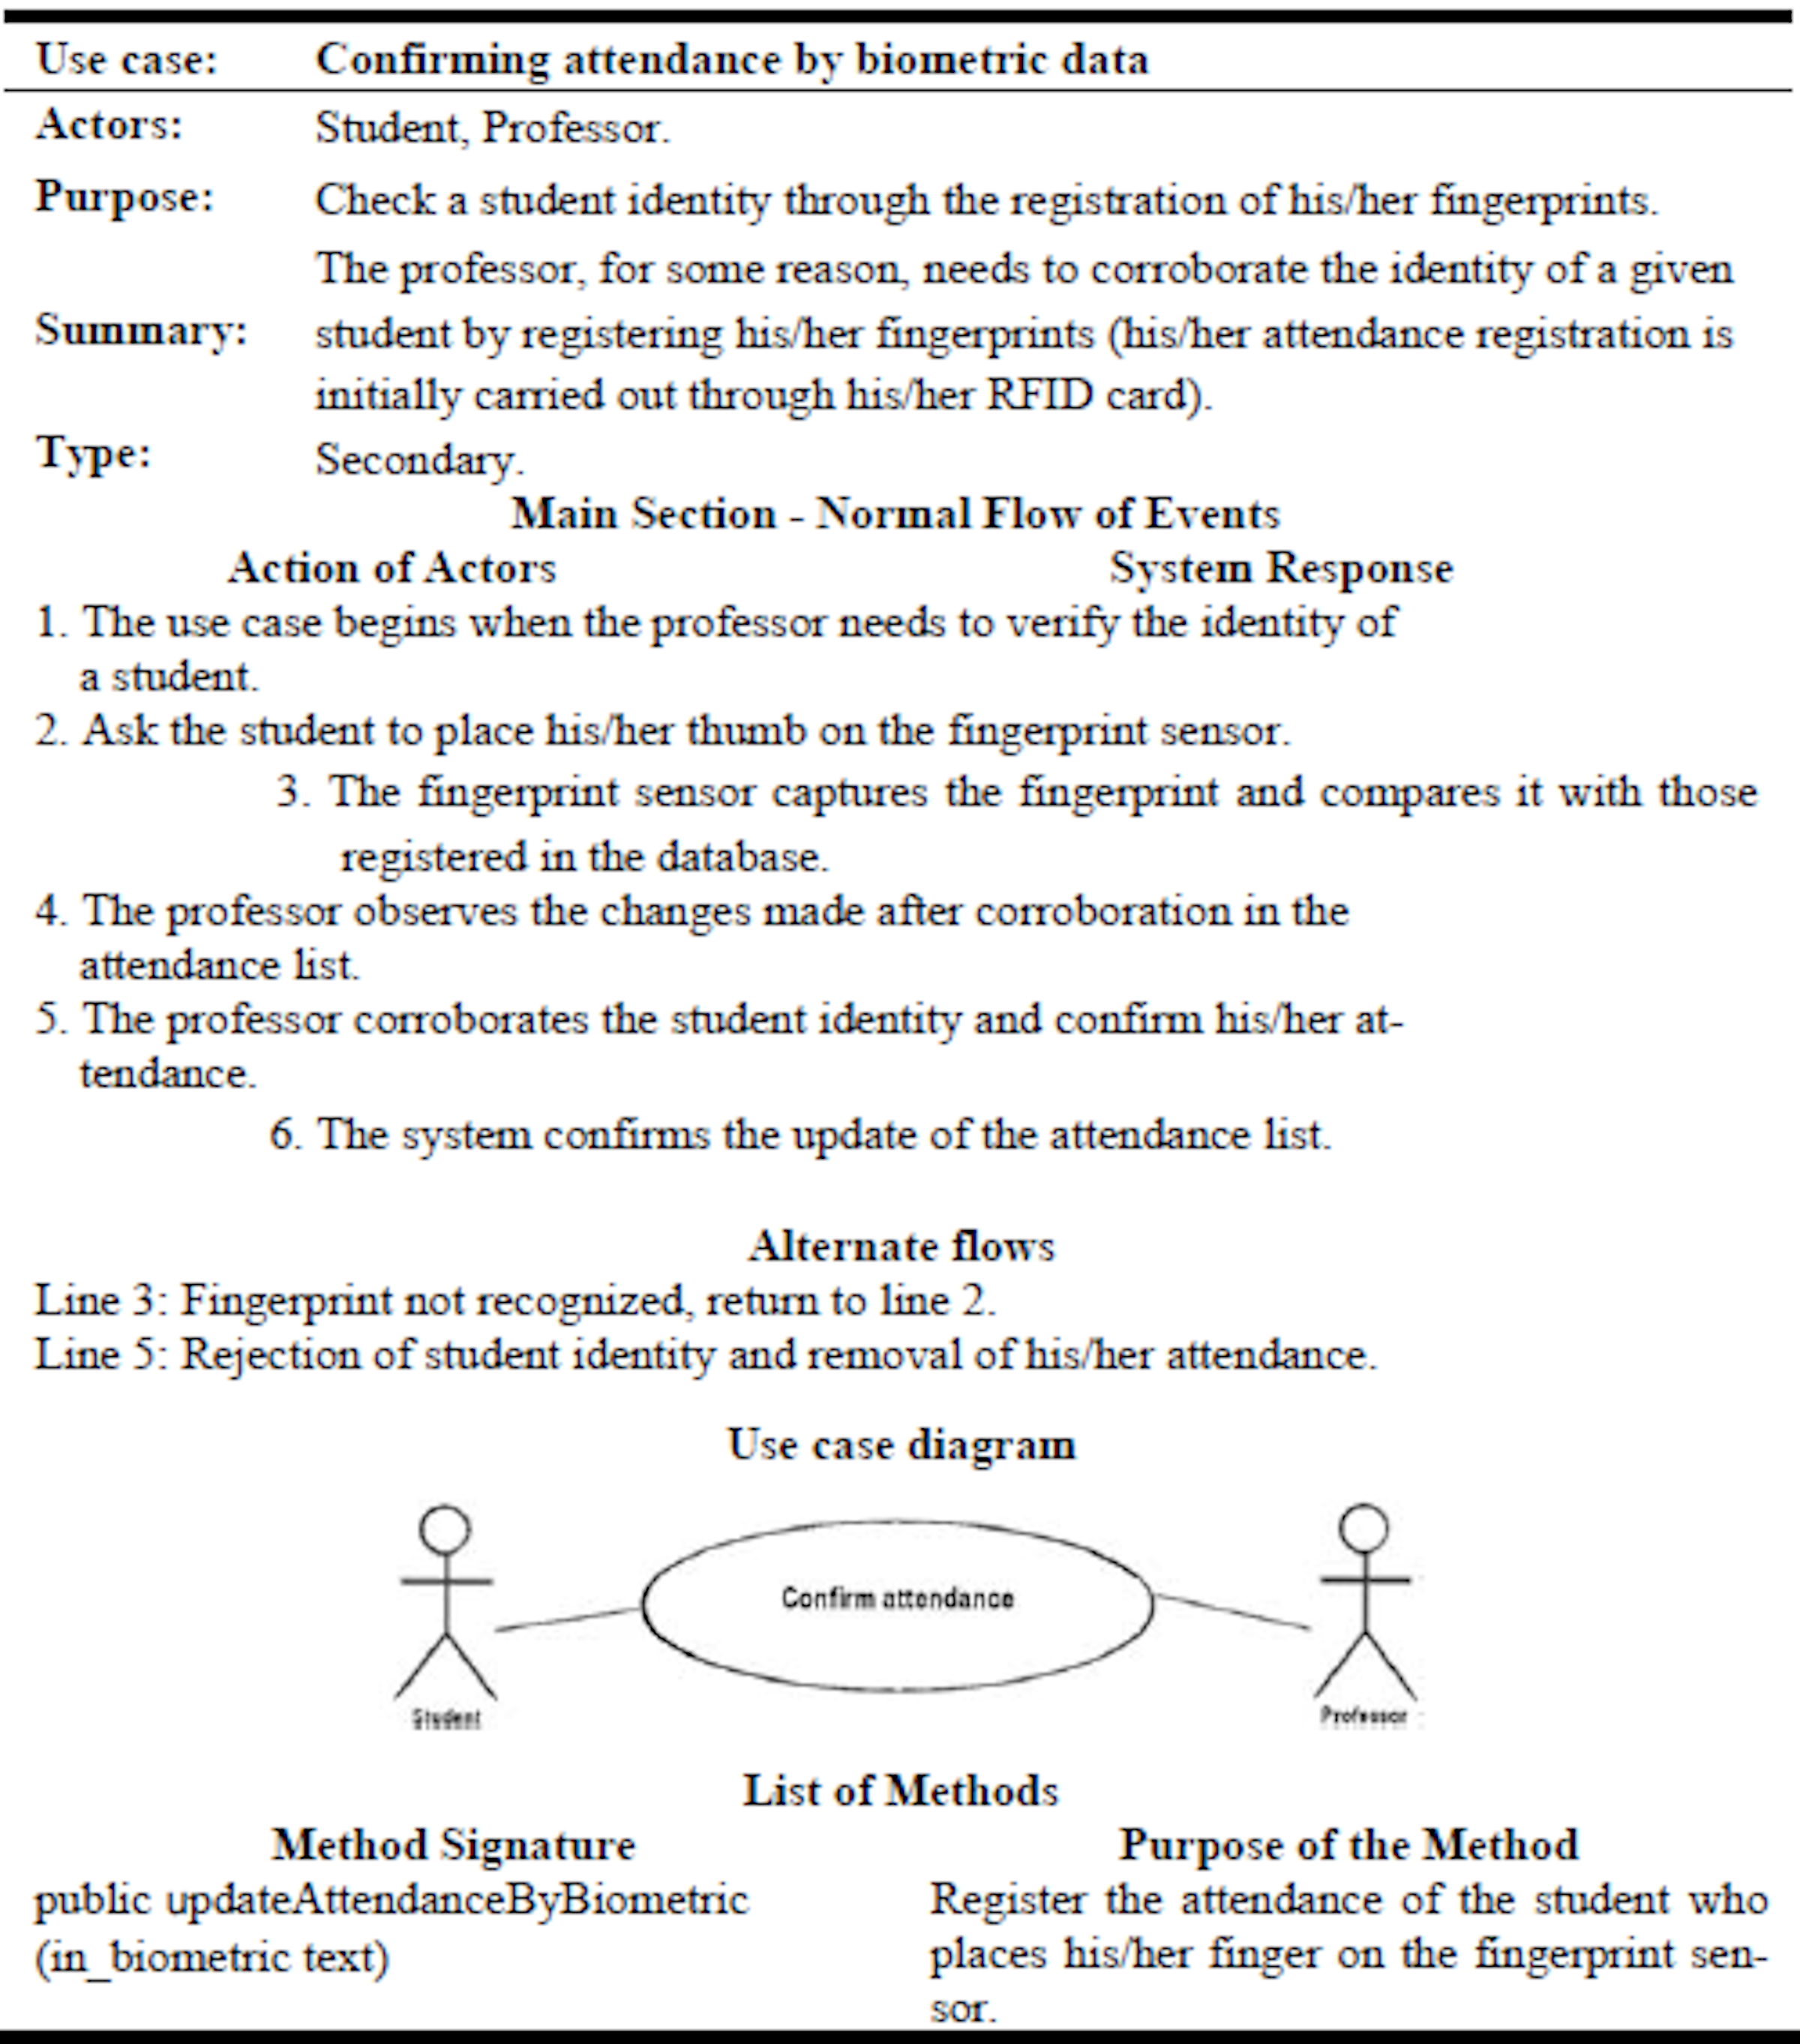
\includegraphics[scale=0.65]{useCase.png}
    %%        \caption{Confirming attendance use case.}
    %%        \label{fig:useCase}
    %%    \end{figure}
    %%\end{frame}
    
     \begin{frame}{Stage 4: Model Generation and Adaptation}
        \begin{block}{}
            In this phase, the class diagram was created, considered one of the most important in the construction of systems, as it serves to represent the architecture of a system, collecting the classes of objects and their relationships involved.\\
            The class diagram was used to better understand the structure of the data to be handled in SISGERA, and also, using the appropriate tools, it was used to generate the database and part of the necessary code.
        \end{block}
    \end{frame}
    
    \begin{frame}{Stage 5: Test generation}
            Below are the tests for the functional requirements related to SISGERA functionality corresponding to keeping both the classroom lights and the equipment off when nobody is in the classroom.
            \begin{itemize}
                \item A professor, who is scheduled to teach a lesson in classroom FCI-008 on Mondays at 10:30, arrives on the correct day but at 10:00. The system informs her/him that it is not time for her/his class and keeps everything turned off.
                \item A person who does not teach in classroom FCI-008, goes to this classroom. The system informs her/him that s/he has no classes scheduled in classroom FCI-008.
                \begin{itemize}
                    \item When leaving the classroom, both equipment and lights are turned on. The system turns off the lights and equipment.
                    \item When leaving the classroom, only the lights are on. The system turns off the lights, and the equipment remains off.
                    \item Before leaving the classroom, lights and equipment are manually turned off. Lights and equipment remain off.
                    \item When leaving the classroom, only the air conditioning is on. The system turns off the air conditioning, and the lights and video projector remain off.
                \end{itemize}
            \end{itemize}
    \end{frame}
    
    \begin{frame}{Stage 6 and 8}
        \begin{block}{Stage 6: Software generation}
            As mentioned in TDDM4IoTS, this process can be manual or automatic. For the automatic generation of the software, Visual Paradigm was used. Visual Paradigm generated a file for each class with its definition, including its attributes and methods, to be used in the mobile application. 100\% of the Arduino code and the rest of the business logic code was written by the development team.\\
            \textbf{Stage 7: Model refinement}\\
            This stage was not necessary because of the size of the project and the developers' mastery of the domain. This is foreseen by the authors of TDDM4IoTS.
        \end{block}
        
        \begin{block}{Stage 8: Software Refinement}
            This stage of TDDM4IoTS was executed only once, after obtaining the mobile application software for SISGERA. It was not necessary to refactor the device configuration software, as it was written by only one of the development team members, considering from the beginning the guidelines to obtain a clean code.
        \end{block}
    \end{frame}
    
    \begin{frame}{Stage 9: Hardware and software deployment}
        \textbf{The device} was deployed as determined in the environment analysis. It was deployed in the classroom, connecting directly to the public power supply without the need for a battery, a router was installed to fix the WiFi signal with good quality.\\
        \textbf{The mobile application} was installed on the smartphones of the teachers who tested the application.
        Teachers can request a classroom for a process they need to carry out, such as a meeting with students about pre-professional practice, tutorials, socialisation of rules or regulations, or even to make up a class session that has been missed. The regular classes of the subjects must be uploaded from the university's academic management system. However, for the tests, they had to be entered one by one, just like the students' lists.
        In addition, the mobile application can be used to control all environmental devices such as lights, air conditioner, video projector, and of course the door unlocking.
    \end{frame}
    
    \begin{frame}{Stage 10: Deliverable assessment}
        \begin{block}{SISGERA assessment}
            The usability evaluation of SISGERA was done along 5 weeks only by professors. At the initial stage, there were some negative comments and 11 a rating of 3 out of 10 for the system. Following these results, more professors were involved in the design of the mobile application interfaces, to implement improvements. Those improvements resulted in 100\% acceptance by professors.
        \end{block}
        \begin{block}{Stage 11: Maintenance}
            SISGERA is a prototype, but considering the improvements made by the teachers' comments, maintenance was not carried out as it is not a production system. However, it is planned to put it into production for a more exhaustive evaluation and to consider the maintenance stage and analyse the scalability feature (increase or remove components to control more or less equipment in the environment).
        \end{block}
    \end{frame}
    
    \begin{frame}{Conclusion}
            \begin{itemize}
                \item We have presented SISGERA, an IoTS for classroom access control and resource management. It uses facial recognition for professors, and fingerprint recognition and RFID for students as user authentication methods.
                \item Facial and fingerprint recognition are more secure authentication methods than traditional methods.
                \item The combination of RFID authentication and fingerprint recognition as identification methods can be used to deter students from identity theft.
                \item SISGERA is designed to be replicated in different classrooms as a distributed system.
                \item TDDM4IoTS is an effective guide for IoTS developers, especially for those who do not have sufficient experience in IoTS development.
                \item End-users should maintain a dedicated involvement in the development of the IoTS, especially in the design of its user interfaces.
                TDDM4IoTS encourages user participation from the earliest stages of IoTS development.
                \item As future work, the usability of the application by students and the energy consumption of two different classrooms, with and without the SISGERA system, respectively, will be evaluated.
            \end{itemize}
    \end{frame}
\end{document}



